% Version 3 October 2023
% Springer Nature sn-jnl template (cleaned for WSInsight manuscript)

\documentclass[sn-mathphys-num]{sn-jnl}% Math and Physical Sciences Numbered Reference Style

%%%% Standard Packages
\usepackage{graphicx}%
\usepackage{amsmath,amssymb,amsfonts}%
\usepackage{amsthm}%
\usepackage{mathrsfs}%
\usepackage[title]{appendix}%
\usepackage{textcomp}%
\usepackage{manyfoot}%
\usepackage{listings}%
%\usepackage{svg}% only needed when \defmysvgtype is svg
\usepackage{subcaption}%
\usepackage{algorithm}%
\usepackage[noend]{algpseudocode}%
\usepackage{xcolor}%
\usepackage{environ}%
\usepackage{hyperref}%
\usepackage{booktabs}%
\usepackage{multirow}%
\usepackage{tabularx}%
\usepackage{array}%
\usepackage{makecell}%
\usepackage{ifthen}%
\usepackage{xparse}%

%%%%%=============================================================================%%%%

%\def\defnpjarticletype{generic}%
\def\defnpjarticletype{npjmanuscript}%
%\def\defnpjarticletype{npjmarkup}%
%\def\defnpjarticletype{npjfinal}%

%%%%%=============================================================================%%%%
\ifthenelse{\equal{\defnpjarticletype}{generic}}%
{%
	%\usepackage[nofiglist]{endfloat}%
	%\usepackage{endfloat}%
	\pagenumbering{gobble}
	%\usepackage{lineno}%
	%\linenumbers%
	\def\defnpjcaptiontype{show}%
	\def\defnpjmarkup{off}%
}%
	
\ifthenelse{\equal{\defnpjarticletype}{npjmanuscript}}{%
	\usepackage{endfloat}%
	\pagenumbering{gobble}%
	\usepackage{lineno}%
	\linenumbers%
	\def\defnpjcaptiontype{hide}%
	\def\defnpjmarkup{off}%
}{}%

\ifthenelse{\equal{\defnpjarticletype}{npjmarkup}}{%
	\usepackage[nofiglist]{endfloat}%
	\usepackage{lineno}%
	\linenumbers%
	\def\defnpjcaptiontype{show}%
	\def\defnpjmarkup{on}%
}{}%

\ifthenelse{\equal{\defnpjarticletype}{npjfinal}}{%
	\usepackage[nomarkers,nofiglist]{endfloat}%
	\pagenumbering{gobble}%
	\def\defnpjcaptiontype{show}%
	\def\defnpjmarkup{off}%
}{}%

%%%%%=============================================================================%%%%

\ifthenelse{\equal{\defnpjcaptiontype}{hide}}{%
	\usepackage[labelformat=empty]{caption}%
}{}%

\NewDocumentCommand{\npjcaption}{m}{%
	\ifthenelse{\equal{\defnpjcaptiontype}{show}}%
	{\caption{#1}}%
	{\caption[#1]{}}%
}%

%%%%%=============================================================================%%%%

\NewDocumentCommand{\npjmarkup}{m}{%
	\ifthenelse{\equal{\defnpjmarkup}{on}}%
	{{\color{red}#1}}%
	{#1}%
}%

\NewEnviron{npjmarkupenv}{%
	\ifthenelse{\equal{\defnpjmarkup}{on}}%
	{\color{red}\BODY}%
	{\BODY}%
}%

%%%%%=============================================================================%%%%
%%% Using SVG or PDF, uncomment below def accordingly.

% \def\defmysvgtype{svg}
\def\defmysvgtype{pdf}

\NewDocumentCommand{\includemysvg}{O{} m}{%
	\ifthenelse{\equal{\defmysvgtype}{svg}}%
	{\includesvg[#1]{#2}}%
	{\includegraphics[#1,type=pdf,ext=.pdf,read=.pdf]{svg-inkscape/#2_svg-tex}}%
}

%%%%%=============================================================================%%%%

\makeatletter%
\def\BState{\State\hskip-\ALG@thistlm}%
\algnewcommand\algorithmicforeach{\textbf{for each}}%
\algdef{S}[FOR]{ForEach}[1]{\algorithmicforeach\ #1\ \algorithmicdo}%
\renewcommand{\Function}[2]{%
	\csname ALG@cmd@\ALG@L @Function\endcsname{#1}{#2}%
	\def\jayden@currentfunction{#1}%
}%
\newcommand{\funclabel}[1]{%
	\@bsphack
	\protected@write\@auxout{}{\string\newlabel{#1}{{\jayden@currentfunction}{\thepage}}}%
	\@esphack
}%
\makeatother%

%%%%%=============================================================================%%%%
%% Theorem styles

\theoremstyle{thmstyleone}%
\newtheorem{theorem}{Theorem}%
\newtheorem{proposition}[theorem]{Proposition}%

\theoremstyle{thmstyletwo}%
\newtheorem{example}{Example}%
\newtheorem{remark}{Remark}%

\theoremstyle{thmstylethree}%
\newtheorem{definition}{Definition}%

\raggedbottom
\unnumbered% uncomment this for unnumbered level heads

%%%%%=============================================================================%%%%

\begin{document}%
	
	\title[WSInsight]{WSInsight as a cloud-native pipeline for multi-scale whole-slide image analysis from patch-level classification to single-cell resolution}
	
	\newbox{\orcid}\sbox{\orcid}{
\includegraphics[scale=0.06]{orcid.pdf}}
	
	\author*[1]{\href{https://orcid.org/0000-0002-3837-8135}{\usebox{\orcid}\hspace{1mm}\fnm{Chao-Hui} \sur{Huang}}}
	\email{chao-hui.huang@pfizer.com}
	\author[1]{\href{https://orcid.org/0000-0003-4638-0144}{\usebox{\orcid}\hspace{1mm}\fnm{Oluwamayowa E.} \sur{Awosika}}}
	\author[1]{\href{https://orcid.org/0000-0003-1365-5172}{\usebox{\orcid}\hspace{1mm}\fnm{Diane} \sur{Fernandez}}}
	
	\affil*[1]{\orgdiv{Oncology Research \& Development}, \orgname{Pfizer Inc.},
		\orgaddress{\street{10777 Science Center Dr.}, \city{San Diego},
			\postcode{92121}, \state{CA}, \country{USA}}}
	
	\abstract{
		Digital pathology has increasingly embraced deep learning for large-scale tissue analysis, yet most workflows remain confined to local execution and patch-level inference. Here we present WSInsight, an open-source, cloud-native pipeline that unifies patch-level classification and single-cell inference on whole-slide images within a single reproducible framework. Building on the WSInfer ecosystem, WSInsight adds end-to-end nuclei segmentation via CellViT, HoVer-Net, and StarDist--ResNet50; introduces graph-based spatial analytics including neighborhood composition analysis and object-to-region spatial registration; and provides native access to cloud-hosted slides through Amazon S3 and NCI Genomic Data Commons manifests. Standardized outputs in GeoJSON and OME-CSV integrate directly with QuPath and OMERO+. Applied to 1{,}061 TCGA breast-cancer slides, WSInsight processes each whole-slide image in approximately 23 seconds on an enterprise GPU workstation, demonstrating scalability for multi-institutional cohort studies.
	}
	
	\keywords{Whole-slide image, cloud-native, digital pathology, deep learning, nuclei segmentation, spatial analysis, multi-scale inference}
	
	\maketitle
	
	%---------------------------------------
	% Introduction
	%---------------------------------------
	
%	\section{Summary}
%	\label{sec:summary}
	
	The digitization of glass slides into high-resolution whole-slide images (WSIs) has created new opportunities for deep learning--based tissue analysis, yet most existing frameworks remain confined to local, patch-level workflows that are difficult to reproduce or deploy across institutions \cite{Gupta:2019, Echle:2020, Laak:2021}. Open-source tools such as WSInfer \cite{Kaczmarzyk:2024}, TIA Toolbox \cite{Pocock:2022}, SlideFlow \cite{Dolezal:2024}, MONAI \cite{Cardoso:2022}, and PHARAOH \cite{Faust:2024} have lowered technical barriers by standardizing model configuration and inference, but none provides a unified cloud-native pipeline that spans patch-level classification, single-cell nuclei analysis, and graph-based spatial profiling. A comparative overview of these tools is provided in Table~\ref{tab:feature_comparison}.
	
	Here we introduce WSInsight, an end-to-end, cloud-native pipeline that extends the WSInfer paradigm to multi-scale whole-slide analysis (Fig.~\ref{fig:diagram}). WSInsight is fully backward-compatible with the WSInfer Model Zoo and additionally supports end-to-end nuclei segmentation and cell-type classification via CellViT \cite{Horst:2024}, HoVer-Net \cite{Graham:2019}, and StarDist--ResNet50 \cite{Schmidt:2018}. Beyond inference, WSInsight introduces graph-based spatial analytics---including neighborhood composition analysis and object-to-region spatial registration---enabling quantitative characterization of the tumor microenvironment at single-cell resolution. The pipeline natively accesses cloud-hosted WSIs through Amazon S3 and NCI Genomic Data Commons (GDC) manifests \cite{TheCancerGenomeAtlasProgramTCGA, CloudObjectStorage--AmazonS3--AmazonWebServices}, produces standardized outputs in GeoJSON for QuPath \cite{Bankhead:2017} and OME-CSV for OMERO+ \cite{Allan:2012}, and can automatically generate QuPath projects for interactive visualization (Fig.~\ref{fig:results}).
	%---------------------------------------
	% Figures
	%---------------------------------------
	
	\begin{figure*}[tb!]%
		\centering%
		\includemysvg[width=1\linewidth]{diagram.drawio}%
		\npjcaption{WSInsight provides an end-to-end, cloud-native workflow for whole-slide image analysis. \textbf{a} WSIs are accessed from cloud or local storage. \textbf{b} A QC-based ROI generator identifies tissue regions, and WSInsight performs patch-level classification and single-cell prediction using models from the WSInfer/WSInsight Model Zoo. \textbf{c} Outputs—region-level probability maps and cellular predictions—are visualized in QuPath and OMERO+ for integrated tissue interpretation.}%
		\label{fig:diagram}%
	\end{figure*}
	
	\begin{figure*}[tb!]%
		\centering%
		\begin{subfigure}[t]{0.5\textwidth}%
			\centering%
			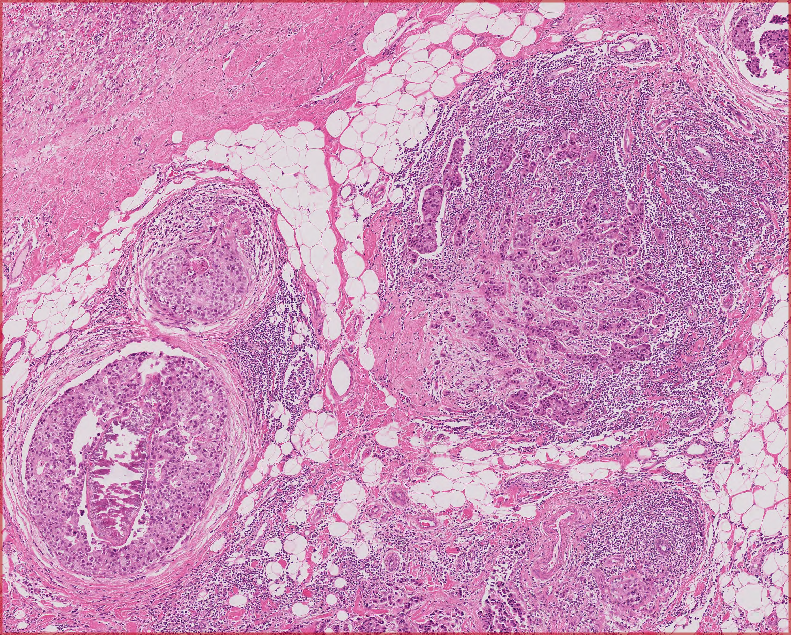
\includegraphics[height=1.75in]{roi-hne.png}%
			\caption{}%
		\end{subfigure}%
		\\%
		\begin{subfigure}[t]{0.5\textwidth}%
			\centering%
			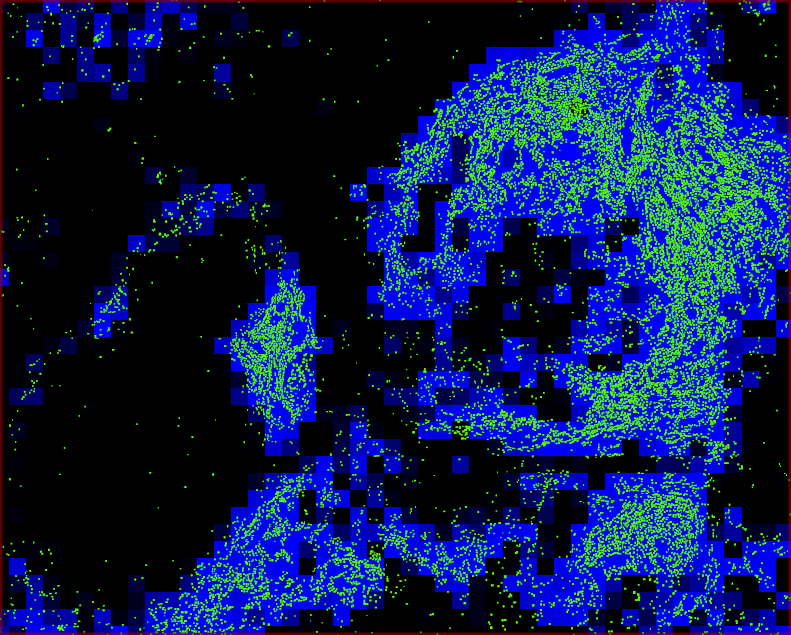
\includegraphics[height=1.75in]{roi-lympho-immune.png}%
			\caption{}%
		\end{subfigure}%
		\begin{subfigure}[t]{0.5\textwidth}%
			\centering%
			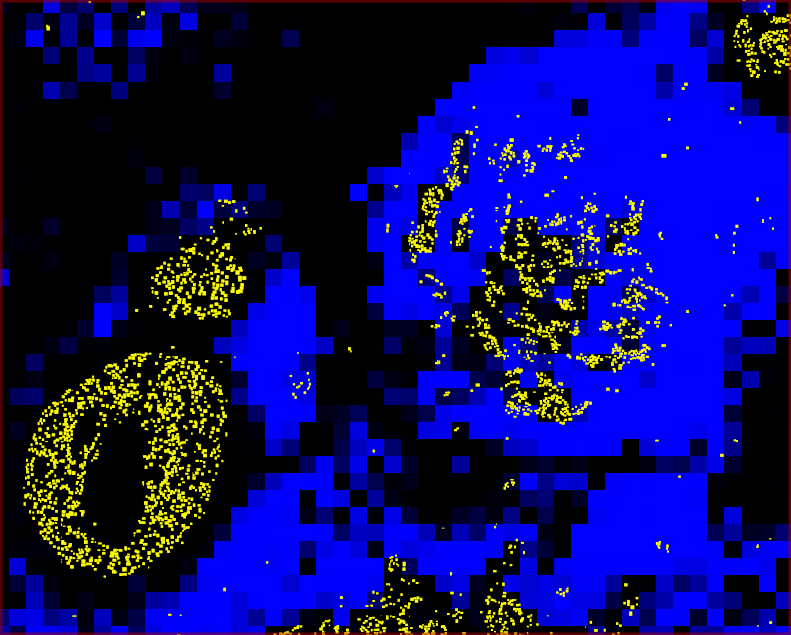
\includegraphics[height=1.75in]{roi-lympho-neoplastic.png}%
			\caption{}%
		\end{subfigure}%
		\\%
		\begin{subfigure}[t]{0.5\textwidth}%
			\centering%
			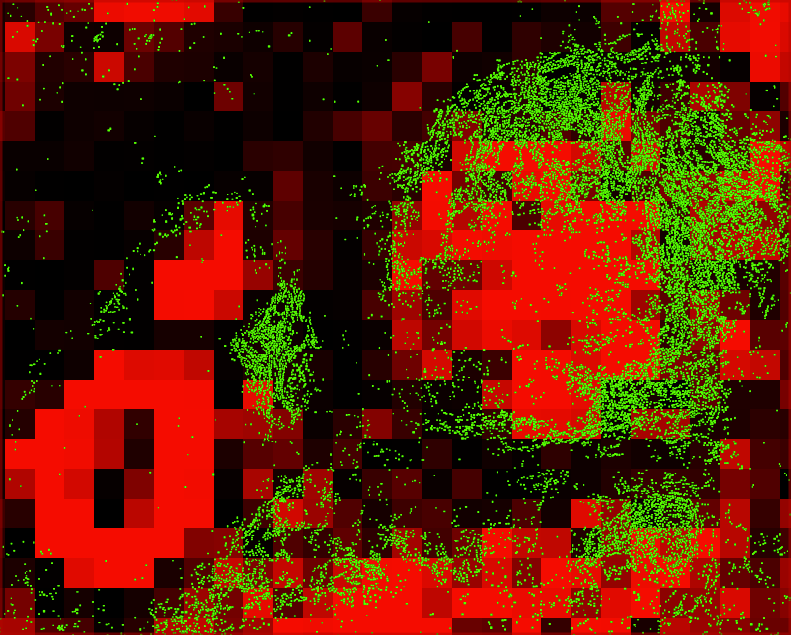
\includegraphics[height=1.75in]{roi-tumor-immune.png}%
			\caption{}%
		\end{subfigure}%
		\begin{subfigure}[t]{0.5\textwidth}%
			\centering%
			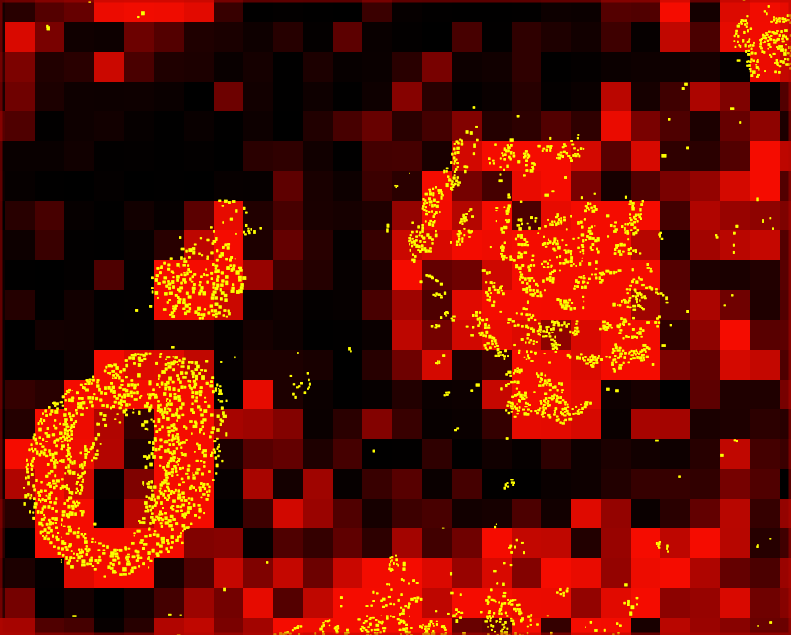
\includegraphics[height=1.75in]{roi-tumor-neoplastic.png}%
			\caption{}%
		\end{subfigure}%
		\npjcaption{Integrative patch-level and single-cell inference on breast cancer H\&E tissue.
			\textbf{a}, Representative hematoxylin–eosin (H\&E) region of interest (ROI).
			\textbf{b}-\textbf{e}, WSInsight multi-scale inference combining patch-level and cell-resolved predictions from the WSInfer/WSInsight Model Zoo. Patch-based models (breast-tumor-resnet34.tcga-brca and lymphnodes-tiatoolbox-resnet50.patchcamelyon) generate heatmaps of tumor-region probability (red) and lymphocyte aggregation (blue). Cell-level predictions from CellViT-SAM-H-x40 identify inflammatory immune cells (green) and neoplastic epithelial cells (yellow) at single-cell resolution.
			Together, these overlays reveal local tumor architecture, immune infiltration, and spatially organized microenvironmental structure.}%
		\label{fig:results}%
	\end{figure*}%
	
	%---------------------------------------
	% Results
	%---------------------------------------
	
	\section{Results}
	\label{sec:results}
	
	\subsection{Multi-scale inference}
	
	To illustrate WSInsight's multi-scale capability, we applied both patch-level and single-cell models to H\&E whole-slide images from TCGA-BRCA (Fig.~\ref{fig:results}). Patch-level models from the WSInfer/WSInsight Model Zoo---breast-tumor-resnet34.tcga-brca \cite{Le:2020} and lymphnodes-tiatoolbox-resnet50.patchcamelyon \cite{Veeling:2018,Pocock:2022,Litjens:2018}---produce heatmaps of tumor-region probability and lymphocyte aggregation. Simultaneously, CellViT-SAM-H-x40 \cite{Horst:2024} resolves individual nuclei and classifies them into inflammatory, neoplastic, epithelial, and connective subtypes. When overlaid, the patch- and cell-resolved outputs provide a coherent, multi-resolution view of the tumor microenvironment, enabling quantitative assessment of immune--tumor interactions and spatial organization within pathologist-defined regions.
	
	\subsection{Runtime performance}
	
	We evaluated WSInsight in two representative environments: one enterprise-grade workstation equipped with a Quadro RTX 8000 GPU running Red Hat Linux, and one consumer-grade system with an RTX 2080 Ti GPU under Windows Subsystem for Linux (Windows 11 with Debian 12). In both settings, we used the breast-tumor-resnet34.tcga-brca model from the WSInfer/WSInsight Model Zoo, applied to whole-slide images from the TCGA repository. The model operates on $350 \times 350$ pixel patches at 0.25~\textmu m per pixel.
	
	In the enterprise environment, analysis of 1{,}061 WSIs completed in 6~h~46~min---equivalent to approximately 23~seconds per WSI (median tissue area = 173~mm\textsuperscript{2}). In the consumer environment, we applied the same configuration to 30 WSIs, a subset of the larger cohort. The total runtime was 14~min~17~s, or about 29~seconds per WSI (median tissue area = 179~mm\textsuperscript{2}).
	
	These benchmarks demonstrate that WSInsight maintains high performance across heterogeneous compute environments, while its cloud-native I/O layer allows the same workflows to be executed directly on slides stored in S3 buckets or accessed through GDC manifests without requiring local staging. WSInsight's adaptive worker optimizer automatically tunes the number of data-loading workers based on available CPU cores, GPU memory, and system RAM, further ensuring efficient utilization of available hardware without manual configuration.

	\subsection{Feature comparison}

	Table~\ref{tab:feature_comparison} compares WSInsight with five related open-source frameworks across seven capability axes. WSInfer \cite{Kaczmarzyk:2024} pioneered reproducible patch-level inference with a curated Model Zoo but does not support single-cell analysis or cloud-native data access. TIA Toolbox \cite{Pocock:2022} provides rich patch and cell analysis utilities, including graph-based tissue profiling, yet lacks built-in cloud I/O and a standardized model zoo. SlideFlow \cite{Dolezal:2024} emphasizes whole-slide deep learning research with MIL and GAN support but does not include single-cell or spatial profiling. MONAI \cite{Cardoso:2022} offers a broad medical-imaging framework with pathology extensions, though its digital pathology coverage is a subset of its scope. PHARAOH \cite{Faust:2024} focuses on interpretable patch-level classification with attention-based reasoning. WSInsight is the only framework that combines cloud-native storage access (S3 and GDC), backward-compatible Model Zoo support, end-to-end single-cell inference, and graph-based spatial analytics within a single pipeline.

	\begin{table*}[tb!]%
		\centering%
		\scriptsize%
		\npjcaption{Feature comparison of open-source whole-slide image analysis frameworks. \checkmark\ = supported; $\sim$ = partial; -- = not supported.}%
		\label{tab:feature_comparison}%
		\begin{tabular}{l c c c c c c c}%
			\toprule%
			\textbf{Framework} & \makecell{\textbf{Cloud-native}\\\textbf{(S3/GDC)}} & \makecell{\textbf{Patch-level}\\\textbf{inference}} & \makecell{\textbf{Single-cell}\\\textbf{inference}} & \makecell{\textbf{Spatial}\\\textbf{analytics}} & \makecell{\textbf{Model}\\\textbf{Zoo}} & \makecell{\textbf{QuPath/}\\\textbf{OMERO+}} & \makecell{\textbf{End-to-end}\\\textbf{CLI}} \\
			\midrule%
			WSInfer \cite{Kaczmarzyk:2024}  & --          & \checkmark & --          & --          & \checkmark & $\sim$     & \checkmark \\
			TIA Toolbox \cite{Pocock:2022}  & --          & \checkmark & \checkmark  & $\sim$      & --         & --         & $\sim$     \\
			SlideFlow \cite{Dolezal:2024}   & --          & \checkmark & --          & --          & --         & --         & $\sim$     \\
			MONAI \cite{Cardoso:2022}       & --          & \checkmark & $\sim$      & --          & $\sim$     & --         & --         \\
			PHARAOH \cite{Faust:2024}       & --          & \checkmark & --          & --          & --         & --         & $\sim$     \\
			\textbf{WSInsight}              & \checkmark  & \checkmark & \checkmark  & \checkmark  & \checkmark & \checkmark & \checkmark \\
			\bottomrule%
		\end{tabular}%
	\end{table*}%
	
	%---------------------------------------
	% Methods
	%---------------------------------------
	
	\section{Methods}
	\label{sec:methods}
	
	The overall WSInsight workflow is illustrated in Fig.~\ref{fig:diagram}, which outlines its three principal components: whole-slide image acquisition, model inference, and integrative visualization. In Step 1 (WSI acquisition), digital pathology slides can be accessed from either cloud-based repositories such as S3 or TCGA, or from local storage, allowing hybrid deployment across institutional infrastructures. In Step 2 (Inference), WSInsight interfaces with both the WSInfer/WSInsight Model Zoo and user-defined models to perform multi-model, integrative inference over the regions of interest (ROI) generated based on the image quality control component, e.g., HistoQC \cite{Janowczyk:2019}. Predictions from diverse deep learning architectures—such as segmentation, classification, or spatial inference models—are unified into cellular- and region-level probability maps. Finally, Step 3 (Visualization and integrative analysis) enables the outputs to be rendered directly within QuPath and OMERO+, where the cellular and regional predictions can be jointly explored. These interoperable layers support quantitative analysis of immune, epithelial, and neoplastic components, allowing users to derive interpretable spatial features that capture the cellular microenvironment and tissue heterogeneity. Collectively, this workflow highlights WSInsight’s design philosophy: an integrated, cloud–local ecosystem that bridges model execution, visualization, and biological interpretation within a single, reproducible framework.
	
	\subsection{Inference Runtime}
	
	The WSInsight inference runtime performs deep learning–based analysis on WSIs at both the patch and single-cell levels, and is available as a command-line interface and a Python package. The runtime accepts three main inputs: a directory or cloud path containing WSIs, a trained model from the WSInfer/WSInsight Model Zoo or a user-provided model, and an output directory for results. Each WSI is processed through a standardized workflow: tissue regions are detected, subdivided into uniformly sized patches, and analyzed using patch-level classification models or single-cell segmentation and typing models, depending on the selected inference mode.
	
	WSInsight supports a wide range of architectures—including patch-based classifiers, nuclei segmentation networks, and single-cell–level cell-type predictors—allowing multi-scale analysis within a unified framework. 
	The runtime exports outputs in GeoJSON format for direct visualization in QuPath, and in comma-separated value (CSV) format structured to be OMERO+-compatible, facilitating integration into large-scale image management and annotation systems. These interoperable outputs ensure that predictions—whether regional tissue classifications or cell-level annotations—can be visualized, aggregated, and quantitatively analyzed across datasets and computational environments.
	
	\subsection{Spatial Analysis}
	\label{sec:spatial}
	
	WSInsight provides two graph-based spatial analysis modules that operate on single-cell detections to characterize the tumor microenvironment.
	
	\paragraph{Neighborhood composition (ncomp).}
	For each detected cell, WSInsight constructs a cell-adjacency graph via Delaunay triangulation of all cell centroids, with edges pruned beyond a configurable distance threshold (default 25~\textmu m). From this graph, $k$-hop neighborhoods (default $k{=}2$) are computed using sparse matrix exponentiation: $\mathbf{M}^k = (\mathbf{A} + \mathbf{I})^k$, where $\mathbf{A}$ is the symmetric adjacency matrix and $\mathbf{I}$ is the identity matrix. Within each cell's $k$-hop neighborhood, the module tallies the number and proportion of every annotated cell type, producing per-cell feature vectors of neighborhood counts and proportions. These features support downstream clustering, phenotype enrichment analysis, and identification of recurrent cellular niches across the tissue.
	
	\paragraph{Object-to-region spatial registration.}
	The registration module performs a spatial join between cell-level detections and patch-level region predictions. Each cell's centroid is tested against region bounding boxes, and region-level attributes (e.g., tumor probability, tissue class) are propagated to the matching cell record. This enables joint region--cell queries such as ``inflammatory cells within high-probability tumor patches'' without manual alignment.
	
	\subsection{Model Zoo}
	
	The WSInfer/WSInsight Model Zoo provides a curated collection of pretrained deep learning models for digital pathology, hosted on the Hugging Face Hub to support open access and reproducible research. Each model repository includes a model card documenting the model’s purpose, architecture, and training data; pretrained weights serialized in TorchScript; and a standardized configuration file specifying input parameters and inference settings. This unified structure ensures consistent documentation, transparent reuse, and cross-platform portability. A public registry on Hugging Face maintains all verified entries in the zoo.

	WSInsight is fully compatible with the WSInfer Model Zoo, allowing all existing WSInfer patch-level models to run directly within the WSInsight runtime without modification. This backward compatibility enables users to reuse, benchmark, and integrate prior patch-based models alongside new single-cell inference modules within a single, cloud-native pipeline.

	Beyond patch-level inference, WSInsight extends the Model Zoo with single-cell–level H\&E image analysis models, enabling nuclei segmentation, phenotype classification, and spatial context modeling. The current WSInsight single-cell collection centers on three families of architectures: (1) CellViT and HoVer-Net, both trained on the PanNuke dataset; and (2) StarDist–ResNet50, provided here as a pan-tissue model trained on pooled 10x Genomics Xenium single-cell datasets curated manually. These models support high-resolution analysis of tissue organization across tumor, immune, and stromal compartments. A compact comparison of these representative architectures is provided in Table~\ref{tab:wsinsight_models}.

	The PanNuke dataset~\cite{Gamper:2019} comprises 19{,}000 H\&E image tiles from multiple organs, each with expert per-nucleus annotations spanning five morphologic classes (neoplastic, inflammatory, connective, dead, epithelial). These annotations enable supervised training for robust nuclei segmentation and phenotype classification across diverse histologic contexts. Within WSInsight, PanNuke-trained CellViT and HoVer-Net models provide a standardized morphological vocabulary that can be reused across projects and tissue types, and their representative performance characteristics are summarized in Table~\ref{tab:wsinsight_models}.

	To complement these morphology-based models, we additionally assembled a manually curated collection of 10x Genomics Xenium datasets spanning multiple tissue types, as listed in Table~\ref{tbl:10xdataset}. Using QuST~\cite{Huang:2025} to derive cell-level annotations from paired Xenium and H\&E data, we constructed harmonized label vocabularies for each anatomical site, capturing cell types based on their morphologic phenotypes observed under H\&E staining. The annotated cell types include adipocyte, basophil, chondrocyte, endothelial, eosinophil, epithelial, fibroblast\_like, glial, hematologic\_blast, lymphocyte, macrophage\_like, malignant\_epithelial, malignant\_melanocytic, mast\_cell, melanocyte, mesangial, neuron, neutrophil, osteoblast, osteocyte, perivascular, plasma\_cell, and smooth\_muscle. When cellular microenvironmental context is taken into account, additional phenotypes such as basaloid\_progenitor, neuroendocrine, and pericyte may also be identified. These site-specific label sets are summarized in Table~\ref{tbl:10xdatasetlabel}.  
	
	%	For pan-tissue cancer studies, and following the cell-type definitions used in PanNuke, these fine-grained labels can be consolidated into five broader morphologic categories: neoplastic, epithelial, inflammatory, connective, and other. Note that dead (necrotic) cells require additional manual annotation, as most single-cell spatial transcriptomics datasets do not include explicit labels for necrosis.
	
	All Xenium datasets in Table~\ref{tbl:10xdataset} are pooled into a single multi-tissue corpus, and the harmonized label schema in Table~\ref{tbl:10xdatasetlabel} is used to supervise a unified pan-tissue model. This strategy leverages the diversity of available tissues while maintaining a consistent output space for downstream spatial analysis. Together, the extended WSInsight Model Zoo spans patch-level, single-cell, and pan-tissue inference, enabling multi-scale integrative analysis across diverse tissue types and experimental modalities.
	
		\begin{table*}[tb!]%
		\centering%
		\scriptsize%
		\npjcaption{Comparison of representative single-cell models \cite{Horst:2024}.}
		\begin{tabular}{p{2.9cm} p{7cm} p{0.75cm} p{0.75cm}}%
			\toprule%
			\textbf{Method} & \textbf{Architecture and Key Features} & \textbf{mPQ} & \textbf{bPQ} \\
			\midrule%
			\textbf{CellViT} \cite{Horst:2024} &
			Vision Transformer encoder with U-Net style decoder; trained on multi-tissue datasets including PanNuke; supports multi-class nuclear instance segmentation and classification. &
			0.4980 & 0.6793 \\
			\midrule%
			\textbf{HoVer-Net} \cite{Graham:2019} &
			CNN backbone (typically ResNet50) with dual-branch decoder predicting nuclear masks and horizontal/vertical (HoVer) distance maps for improved instance separation. &
			0.4629 & 0.6596 \\
			\midrule%
			\textbf{StarDist–ResNet50} \cite{Schmidt:2018, He:2016} &
			ResNet50 backbone paired with star-convex polygon representation predicting radial distances along fixed rays for nuclei delineation. &
			0.4796 & 0.6692 \\
			\bottomrule%
		\end{tabular}%
		\label{tab:wsinsight_models}%
	\end{table*}%
	
	% ---------- Counter + commands ----------
\newcounter{xeniumdataset}%

\newcommand{\datasetentry}[2]{%
	\refstepcounter{xeniumdataset}%
	\label{dataset:#1}%
	\thexeniumdataset. & #2 \\% 
}%

\newcommand{\datasetref}[1]{\ref{dataset:#1}}%
% ---------------------------------------

\begin{table}[t]%
	\footnotesize%
	\npjcaption{Public datasets provided by 10x Genomics (under the CC-BY 2.0 license).}
	\label{tbl:10xdataset}%
	\begin{tabularx}{\linewidth}{@{}r@{\hspace{0.4em}}>{\raggedright\arraybackslash}X@{}}%
		\toprule%
		% & \textbf{10X Genomics Xenium Dataset} \\
		% \midrule%
		\datasetentry{bone-femur-normal}{Human Bone and Bone Marrow Data with Custom Add-on Panel / Non-diseased Femur Bone}
		\datasetentry{bone-all-marrow}{Human Bone and Bone Marrow Data with Custom Add-on Panel / Acute Lymphoid Leukemia Bone Marrow}
		\datasetentry{bone-marrow-normal}{Human Bone and Bone Marrow Data with Custom Add-on Panel / Non-diseased Bone Marrow}
		\datasetentry{brain-io}{FFPE Human Brain Cancer Data with Human Immuno-Oncology Profiling Panel and Custom Add-on}
		\datasetentry{breast-pan5k}{FFPE Human Breast Cancer with 5K Human Pan Tissue and Pathways Panel plus 100 Custom Genes}
		\datasetentry{breast-entire-1}{FFPE Human Breast using the Entire Sample Area / Replicate 1}
		\datasetentry{breast-entire-2}{FFPE Human Breast using the Entire Sample Area / Replicate 2}
		\datasetentry{breast-predesigned-1}{FFPE Human Breast with Pre-designed Panel / Tissue sample 1}
		\datasetentry{breast-custom-idc}{Xenium FFPE Human Breast with Custom Add-on Panel / Tissue sample 1 (IDC)}
		\datasetentry{breast-custom-1}{FFPE Human Breast with Custom Add-on Panel / Tissue sample 1}
		\datasetentry{breast-predesigned-2}{FFPE Human Breast with Pre-designed Panel / Tissue sample 2}
		\datasetentry{breast-custom-2}{FFPE Human Breast with Custom Add-on Panel / Tissue sample 2}
		\datasetentry{cervix-pan5k}{FFPE Human Cervical Cancer with 5K Human Pan Tissue and Pathways Panel plus 100 Custom Genes}
		\datasetentry{colon-cancer-preview}{Human Colon Preview Data (Xenium Human Colon Gene Expression Panel) / Cancer / pre-designed + add-on panel}
		\datasetentry{colon-normal-preview}{Human Colon Preview Data (Xenium Human Colon Gene Expression Panel) / Non-diseased / pre-designed panel}
		\datasetentry{colon-colorectal-io}{FFPE Human Colorectal Cancer Data with Human Immuno-Oncology Profiling Panel and Custom Add-on}
		\datasetentry{heart-mt}{Human Heart Data with Xenium Human Multi-Tissue and Cancer Panel}
		\datasetentry{kidney-cancer-preview}{Human Kidney Preview Data (Xenium Human Multi-Tissue and Cancer Panel) / Kidney Cancer (PRCC)}
		\datasetentry{kidney-normal-preview}{Human Kidney Preview Data (Xenium Human Multi-Tissue and Cancer Panel) / Non-diseased Kidney}
		\datasetentry{kidney-rcc-in-situ}{Xenium In Situ Gene and Protein Expression data for FFPE Human Renal Cell Carcinoma}
		\datasetentry{liver-cancer}{Human Liver Data with Xenium Human Multi-Tissue and Cancer Panel / Liver cancer}
		\datasetentry{liver-normal}{Human Liver Data with Xenium Human Multi-Tissue and Cancer Panel / Non-diseased}
		\datasetentry{lung-prime-exp2}{Post-Xenium Technical Note: Xenium v1 and Xenium Prime 5K for FFPE Human Lung Cancer / Experiment 2/ Xenium Prime 5K}
		\datasetentry{lung-io}{FFPE Human Lung Cancer Data with Human Immuno-Oncology Profiling Panel and Custom Add-on}
		\datasetentry{lung-v1-exp1}{Post-Xenium Technical Note: Xenium v1 and Xenium Prime 5K for FFPE Human Lung Cancer / Experiment 1 / Xenium v1}
		\datasetentry{lung-seg}{Preview Data: FFPE Human Lung Cancer with Xenium Multimodal Cell Segmentation}
		\datasetentry{lymph-node-pan5k}{Preview Data: FFPE Human Lymph Node with 5K Pan Tissue and Pathways Panel}
		\datasetentry{ovary-pan5k}{FFPE Human Ovarian Cancer with 5K Human Pan Tissue and Pathways Panel plus 100 Custom Genes}
		\datasetentry{ovary-io}{FFPE Human Ovarian Cancer Data with Human Immuno-Oncology Profiling Panel and Custom Add-on}
		\datasetentry{pancreas-cancer}{Pancreatic Cancer with Xenium Human Multi-Tissue and Cancer Panel}
		\datasetentry{pancreas-pdac-io}{FFPE Human Pancreatic Ductal Adenocarcinoma Data with Human Immuno-Oncology Profiling Panel}
		\datasetentry{pancreas-seg}{FFPE Human Pancreas with Xenium Multimodal Cell Segmentation}
		\datasetentry{prostate-preview}{Preview Data: FFPE Human Prostate Adenocarcinoma with 5K Human Pan Tissue and Pathways Panel}
		\datasetentry{skin-melanoma}{Preview Data: FFPE Human Skin Primary Dermal Melanoma with 5K Human Pan Tissue and Pathways Panel}
		\datasetentry{skin-preview}{Human Skin Preview Data (Xenium Human Skin Gene Expression Panel)}
		\datasetentry{skin-mt-1}{Human Skin Data with Xenium Human Multi-Tissue and Cancer Panel / Sample 1}
		\datasetentry{skin-mt-2}{Human Skin Data with Xenium Human Multi-Tissue and Cancer Panel / Sample 2}
		\datasetentry{skin-preview-addon}{Human Skin Preview Data (Xenium Human Skin Gene Expression Panel with Custom Add-On)}
		\datasetentry{tonsil-follicular}{Human Tonsil Data with Xenium Human Multi-Tissue and Cancer Panel / Follicular lymphoid hyperplasia}
		\datasetentry{tonsil-reactive}{Human Tonsil Data with Xenium Human Multi-Tissue and Cancer Panel / Reactive follicular hyperplasia}
		\bottomrule%
	\end{tabularx}%
\end{table}%
	
	\begin{table}[t]%
		\footnotesize%
		\setlength{\tabcolsep}{6pt}%
		\renewcommand{\arraystretch}{1.2}%
		\npjcaption{Available single-cell annotations based on 10x Genomics public datasets.}%
		\label{tbl:10xdatasetlabel}%
		\begin{tabularx}{\linewidth}{p{9em} >{\raggedright\arraybackslash}X p{2.5cm}}%
			\toprule%
			\textbf{Tissue Site} & \textbf{Labels} & \textbf{Training Dataset (see Table~\ref{tbl:10xdataset})} \\
			\midrule[0.08em]%
			bone\hspace{9em}(incl. bone marrow) & adipocyte, chondrocyte, endothelial, fibroblast\_like, hematologic\_blast, lymphocyte, macrophage\_like, malignant\_epithelial, mast\_cell, neutrophil, osteoblast, osteocyte, pericyte &  \datasetref{bone-femur-normal}, \datasetref{bone-all-marrow}, \datasetref{bone-marrow-normal}\\
			\cmidrule(lr){1-3}
			brain & fibroblast\_like, glial, lymphocyte, macrophage\_like, neutrophil, pericyte &  \datasetref{brain-io}\\
			\cmidrule(lr){1-3}
			breast & adipocyte, endothelial, epithelial, fibroblast\_like, lymphocyte, macrophage\_like, malignant\_epithelial, mast\_cell, pericyte, plasma\_cell & \datasetref{breast-pan5k}, \datasetref{breast-entire-1}, \datasetref{breast-entire-2}, \datasetref{breast-predesigned-1}, \datasetref{breast-custom-idc}, \datasetref{breast-custom-1}, \datasetref{breast-predesigned-2}, \datasetref{breast-custom-2} \\
			\cmidrule(lr){1-3}
			cervix  & basaloid\_progenitor, endothelial, epithelial, fibroblast\_like, lymphocyte, macrophage\_like, malignant\_epithelial, pericyte, smooth\_muscle & \datasetref{cervix-pan5k} \\
			\cmidrule(lr){1-3}
			colorectal  & basaloid\_progenitor, basophil, endothelial, eosinophil, epithelial, fibroblast\_like, hematologic\_blast, lymphocyte, macrophage\_like, malignant\_epithelial, mast\_cell, neuron, neutrophil, pericyte, plasma\_cell & \datasetref{colon-cancer-preview}, \datasetref{colon-normal-preview}, \datasetref{colon-colorectal-io} \\
			\cmidrule(lr){1-3}
			heart & basophil, cardiomyocyte, endothelial, fibroblast\_like, lymphocyte, macrophage\_like & \datasetref{heart-mt} \\
			\cmidrule(lr){1-3}
			kidney & endothelial, epithelial, fibroblast\_like, lymphocyte, macrophage\_like, malignant\_epithelial, mesangial, neutrophil, pericyte, perivascular, plasma\_cell & \datasetref{kidney-cancer-preview}, \datasetref{kidney-normal-preview}, \datasetref{kidney-rcc-in-situ} \\
			\cmidrule(lr){1-3}
			liver & endothelial, epithelial, fibroblast\_like, lymphocyte, macrophage\_like, malignant\_epithelial, pericyte, plasma\_cell & \datasetref{liver-cancer}, \datasetref{liver-normal} \\
			\cmidrule(lr){1-3}
			lung & basophil, endothelial, epithelial, fibroblast\_like, hematologic\_blast, lymphocyte, macrophage\_like, malignant\_epithelial, mast\_cell, pericyte, plasma\_cell, smooth\_muscle & \datasetref{lung-prime-exp2}, \datasetref{lung-io}, \datasetref{lung-v1-exp1}, \datasetref{lung-seg} \\
			\cmidrule(lr){1-3}
			lymph node & endothelial, fibroblast\_like, hematologic\_blast, lymphocyte, macrophage\_like, mast\_cell, pericyte, plasma\_cell & \datasetref{lymph-node-pan5k} \\
			\cmidrule(lr){1-3}
			pancreas & endothelial, epithelial, fibroblast\_like, lymphocyte, macrophage\_like, malignant\_epithelial, mast\_cell, neuroendocrine, neutrophil, pericyte, plasma\_cell & \datasetref{pancreas-cancer}, \datasetref{pancreas-pdac-io}, \datasetref{pancreas-seg} \\
			\cmidrule(lr){1-3}
			prostate & endothelial, epithelial, fibroblast\_like, lymphocyte, macrophage\_like, malignant\_epithelial, neutrophil, pericyte, plasma\_cell, smooth\_muscle & \datasetref{prostate-preview} \\
			\cmidrule(lr){1-3}
			skin & basophil, endothelial, epithelial, fibroblast\_like, lymphocyte, macrophage\_like, malignant\_epithelial, malignant\_melanocytic, mast\_cell, melanocyte, neuroendocrine, pericyte, plasma\_cell & \datasetref{skin-melanoma}, \datasetref{skin-preview}, \datasetref{skin-mt-1}, \datasetref{skin-mt-2}, \datasetref{skin-preview-addon} \\
			\cmidrule(lr){1-3}
			tonsil & basophil, endothelial, fibroblast\_like, hematologic\_blast, lymphocyte, macrophage\_like, mast\_cell, pericyte, plasma\_cell & \datasetref{tonsil-follicular}, \datasetref{tonsil-reactive} \\
			\cmidrule(lr){1-3}
			\morecmidrules
			\cmidrule(lr){1-3}
			pan-tissue & neoplastic, epithelial, inflammatory, connective, background
			& all of above \\
			\bottomrule%
		\end{tabularx}%
	\end{table}%
	
	\subsection{Reporting summary}
	
	Further information on research design is available in the Nature Research Reporting Summary linked to this article.
	
	%---------------------------------------
	% Code availability, contributions, etc.
	%---------------------------------------
	
	\section{Code Availability}
	
	The WSInsight framework is open source under the Apache 2.0 license. The source code, container images, and Model Zoo configurations are available at \url{https://github.com/huangch/wsinsight}. %Documentation provides setup guides for cloud, HPC, and local execution, with reproducible examples demonstrating Xenium-trained model usage and integration with HistoQC \cite{Janowczyk:2019}.
	
	\section{Data Availability}
	
	The whole-slide images used for runtime benchmarking were obtained from The Cancer Genome Atlas (TCGA) via the NCI Genomic Data Commons (GDC) portal (\url{https://portal.gdc.cancer.gov}), which is publicly accessible under NIH data-use policies \cite{TheCancerGenomeAtlasProgramTCGA}. The 10x Genomics Xenium single-cell datasets used for StarDist--ResNet50 training are publicly available under the Creative Commons Attribution 2.0 (CC-BY~2.0) license from the 10x Genomics website (\url{https://www.10xgenomics.com/datasets}); the specific datasets are enumerated in Table~\ref{tbl:10xdataset}. All pretrained model weights in the WSInfer/WSInsight Model Zoo are hosted on the Hugging Face Hub at \url{https://huggingface.co/kaczmarj}.
	
	\section{Author Contributions}
	
	C.H.H. conceived and led the WSInsight design and implementation. O.E.A. contributed model validation and dataset curation. D.F. oversaw oncology use cases and biological interpretation. All authors wrote and approved the manuscript.
	
	\section{Competing Interests}
	
	The authors are employees of Pfizer Inc. This work was conducted as part of their employment. The authors declare no other competing interests.
	
	\section{Funding}
	
	Not applicable.
	
	\section{Acknowledgements}
	
	We thank the WSInfer authors, digital pathology and computational biology communities for open-source resources, and acknowledge TCGA and 10x Genomics that enabled this study.
	
	\bibliography{wsinsight-main}
	
\end{document}
